\documentclass{article}

\usepackage[italian]{babel}
\usepackage[autostyle,italian=guillemets]{csquotes}
\usepackage[backend=biber]{biblatex}
\usepackage{todonotes}
\usepackage{graphicx}
\usepackage{hyperref}
\addbibresource{bibliography.bib}

\begin{document}
\title{Convolutional Neural Network for epileptic seizure recognition}
\maketitle

\tableofcontents

\section*{Introduzione}
Il progetto è stato realizzato con lo scopo di attuare delle predizioni di crisi epilettiche su tracciati EEG che registrano le attività del  cervello umano a livello neurale.
La predizione viene effettuata creando una rete neurale allenata per riconoscere le varie crisi presenti.
Queste predizioni vengono eseguite su file .edf (European Data Format) i quali permettono un'archiviazione di segnali biologici e fisici multicanale.
Il tool non solo permette di predirre le crisi presenti in un tracciato EEG, ma dispone di altre funzionalità come la definizione di alcune statistiche che riguardano tutti i segnali e tutti i canali presenti nel tracciato.
Viene fornita all'utente l'opportunità di creare il proprio dataset di allenamento che poi sarà usato sulla rete neurale che esso stesso potrà definirsi. 
Il progetto è stato suddiviso in:
\begin{itemize}
\item studio EEG e teoria delle crisi
\item studio per la creazione del dataset (segnali ictali, preictali e postictali)
\item bilanciamento dataset
\item studio teorico cnn
\item applicazione CNN con relativo allenamento
\item costruzione architettura web con beckend e frontend 
\end{itemize}


\section{Epilessia}
L'epilessia è una malattia neurologica che colpisce circa 50 milioni di persone nel mondo. Essa è caratterizzata da specifici eventi clinici, definiti crisi epilettiche, che si ripetono in modo consecutivo e attivano simultaneamente un grane numero di neuroni generalemente posti in un'area particolare dell'encefalo, detta corteccia celebrale. Quindi questi eventi scaturiti dalle crisi che si verificano alterano la normale attività elettrica dell'encefal, con conseguenze sul comportamento del soggetto colpito, come perdita di conoscenza, movimenti involontari, contrazioni della muscolatura che si tramutano in convulsioni.
Le cause delle crisi epilettiche possono essere diverse, come in caso di patologie, in un trauma cranico, infenzioni SNC (meningite ecc..), ed anche a causa di vari farmaci che possono essere somministrati.
In base all'area di estensione del cervello che è interessata da scariche elettriche anomale, possono presentarvi due tipi di crisi, crisi parziali e crisi generalizzate.
\begin{itemize}
\item Crisi Parziali:  si manifestano convulsioni e alterazioni sensoriali. Esse si suddividono a loro volta da crisi semplici o complesse 
\begin{itemize}
\item Semplici: interessa una piccola regione del cervello, come il lobo temporale o l'ippocampo. questo tipo di crisi spesso precede una crisi peggiore, dove l'anomala attività elettrica coinvolge aree più vaste del cervello.
\item Complessa: Interessa aree più vaste del cervello e non è concentrata solo su alcune di esse. Questo tipo di crisi è più dannosa perchè scaturisce nel soggetto coinvolto una perdita di coscienza.
\end{itemize}
\item Generalizzate: crisi più frequenti rispetto alle parziali, esse vengono generate a causa di un'alterazione dell'attività neuronale di  entrambi gli emisferi.
\end{itemize}
\todo{ quando si può dire di essere affetti da epilessia  }
\todo{ rimedi per l'epilessia, farmaci e se viene curata del tutto o meno   }
\todo{spiegazione EEG tecnica per la registrazione, come funziona, cosa registra e come viene applicata allo scalpo}
 In alcuni casi dopo uno o più episodi di crisi epilettiche il fenomeno può tendere a scomparire per cause naturali senza l'apporto di farmaci per la sua cura. In molti casi però c'è bisogno di una cura effettuata attraverso farmaci, se questi ultimi non dovrebbero essere efficaci c'è bisogno di ricorre a operazioni chirurgiche.
I farmaci risultano efficaci nel 60-70 per cento dei casi, questi non curano l'epilessia ma permettono al soggetto affetto di convivere con questa patologia.
 La diagnosi dell'epilessia viene fatta attraverso diversi strumenti, uno su tutti è l'elettroencefalogramma (EEG). Questo strumento registra le attività elettriche dell'encefalo, poi riprodotte su dei tracciati grafici che contengono diversi tracciati,  che mostrano delle onde, corrispondenti agli elettrodi applicati sullo scalpo del soggetto.
 Attraverso questo strumento è possibile individuare le cause di una crisi epilettica e le alterazioni  elettriche che avvengono all'interno del cervello sia in condizioni normali, di riposo, sia in situazioni di crisi. In base alle caratteristiche del tracciato risultante i medici possono dedurre di che tipo di epilessia si tratta e quale cura è meglio prescrivere. 
https://www.my-personaltrainer.it/salute/epilessia.html


\section{Reti Neurali}
Le reti neurali sono modelli matematici basati su neuroni artificiali ispirati al funzionamento biologico del cervello umano. Inventate intorno alla metà degli anni 80, sono tornate in auge nell'ultimo decennio come strumento di risoluzione in svariati campi, dall'informatica, all'elettronica, alla simulazione. 
Prendendo spunto dal cervello animale, una rete neurale(ANN) è composta da numerosi neuroni connessi fra loro. Ogni connessione, come le sinapsi cerebrali, trasmette un segnale da un neurone all'altro. Il neurone che riceve un segnale può processarlo e inviarlo ai neuroni a cui è a sua volta connesso. Tradizionalmente, un segnale trasmesso tra due neuroni è rappresentato da un numero reale, moltiplicato per un certo peso che indica la forza della connessione. Ogni neurone esegue una somma di tutti i segnali in ingresso, moltiplicandoli per il suo set di pesi. Tale somma viene poi modellata da una funzione di attivazione, tipicamente la sigmoide
$\sigma(x) = {1 \over 1+e^-x}$.\\
In una rete neurale i neuroni sono solitamente distribuiti su più layer, che applicano diverse trasformazioni agli input. I segnali in ingresso viaggiano sequenzialmente dal primo layer (input layer) all'ultimo (Output layer), attraversando un numero n di layer intermedi (Hidden layer).

La peculiarità delle reti neurali rispetto all'utilizzo di sistemi di risoluzione tradizionali è l'apprendimento. Le ANN vengono addestrate per capire come dovranno comportarsi nel momento in cui andranno a risolvere un problema ingegneristico. L'approccio orientato all'apprendimento si basa sui principi del Machine Learning, la disciplina che studia i diversi metodi matematico-computazionali per apprendere informazioni dall'esperienza. Possiamo distinguere quattro principali metodologie di apprendimento:

\begin{itemize}
\item Supervised Learning: la rete riceve un input e il relativo risultato atteso. L'obiettivo è quello di identificare una regola generale che colleghi i dati in ingresso con quelli in uscita.
\item Unsupervised Learning: la rete riceve solo set di dati in input, senza alcuna indicazione del risultato desiderato. Lo scopo è quello di risalire a schemi nascosti tra gli input, in modo da identificarne una struttura logica.
\item Apprendimento per rinforzo: il comportamento del sistema è determinato da una routine di apprendimento basata su ricompensa se l'obiettivo è raggiunto, o punizione se viene commesso un errore.
\item Apprendimento semi-supervised: modello ibrido basato sui primi due, in cui solo ad una parte dei dati in input è associato il rispettivo output atteso.
\end{itemize}

L'allenamento supervisionato, quello implementato in questo progetto, prevede diversi passi:
\begin{itemize}
\item Inizializzazione: il modello viene inizializzato con valori casuali per bias e pesi. 
\item Feed-forward: il modello prende i dati in input e restituisce un output, rappresentante la predizione.
\item Loss function: viene calcolata la differenza tra l'output atteso e quello calcolato dalla rete. Fornisce quindi una metrica sull'accuratezza della rete. \todo{CrossEntropyLoss} Inizialmente la precisione sarà molto bassa. L'obiettivo dell'allenamento è appunto quello di minimizzare il loss per aumentare la precisione della rete. 
\item Differentiation: calcolando la derivata della funzione di loss, vengono identificate le modifiche da applicare ai pesi per diminuire l'errore sul risultato. Lo standard de facto per effettuare tale ottimizzazione è lo \textit{stochastic gradient descent}. Tale metodo prevede che per il calcolo del gradiente (il vettore contenente le derivate perziali della funzione di loss) venga preso solo un sottoinsieme dei valori, in modo da ridurre la complessità del calcolo.  \todo{adam optimizer}
\item Backpropagation and weights update: i valori dei pesi vengono aggiornati, a partire dal layer di output fino ad arrivare al primo layer, per far sì che il loss venga minimizzato. La retropropagazione dell'errore prevede la selezione di una costante rappresentata da un numero decimale molto piccolo, che viene moltiplicato per l'incremento. Facendo questo, i pesi vengono modificati più lentamente in modo da centrare il minimo della funzione di loss.
\end{itemize}

\section{Reti Neurali Convoluzionali}
Il funzionamento delle reti neurali tradizonali è poco efficiente quando deve essere analizzato un numero molto grande di dati. Ogni neurone prevede una connessione con ogni neurone del layer successivo (per questo sono chiamati fully-connected layers). Ciò implica che al crescere della dimensione della rete, cresce inesorabilmente il numero di parametri di cui tener traccia, portando a casi si sovradattamento della rete.

Già dalla fine degli anni 90 i progettisti di reti neurali hanno iniziato ad introdurre dei modelli di reti convoluzionali, che permettono di ridurre di molto la grandezza della rete. Queste sono molto simili alle reti tradizionali: sono anch'esse formate da neuroni e tengono traccia di parametri come funzioni di attivazione e pesi che vengono modificati durante l'apprendimento. La caratteristica differente risiede nei layer convoluzionali di queste reti. Essi sono particolarmente indicati per il riconoscimento di proprietà nell'architettura dei dati in ingresso, che sono trattati come fossero immagini. La convoluzione prende infatti spunto dal funzionamento della corteccia visiva animale. Intuitivamente, un layer convoluzionale ha il compito di riconoscere alcune caratteristiche visive dell'immagine, come contorni, linee, colori ecc.. concentrandosi su piccole porzioni dell'immagine, e non prendendola nel suo complesso come accade neille reti fully-connected. Una volta individuata una caratteristica in una certa sezione dell'immagine, la rete sarà in grado di riconoscerla se dovesse presentarsi in altri punti. In una successione di layer convoluzionali, inoltre, un layer più imparare a riconoscere combinazioni di caratteristiche base individuate nei precedenti strati. Ciò le rende particolarmente adatte alla comprensione di pattern complessi.

Un convolutional layer è generalmente formato da un set di filtri (kernel) della stessa dimensione. Durante la computazione tali filtri vengono applicati ai dati in ingresso, attraverso una moltiplicazione element-wise. I valori della matrice di ogni moltiplicazione element-wise vengono sommati fra loro e restituiti in output.
Un layer convoluzionale è governato da tre parametri:
\begin{itemize}
\item profondità (K): numero di filtri da applicare durante la convoluzione. Questo determinerà infatti la profondità dell'output.
\item stride (S): indica il numero di segnali per cui si vuole traslare il filtro ad ogni spostamento. Uno stride piccolo genera molti più spostamenti, aumentando la dimensione dell'output. 
\item zero-padding (P): segnali settati a zero, aggiunti ai bordi dei segnali di input. Serve spesso per adattare la dimensione dell'input con quella dell'output. Uno strato aggiuntivo di zeri infatti aumenterà la dimensione del vettore di output. 
\end{itemize}

Dato un seti di dati in ingresso (I) la dimensione del volume di output (O) di un livello convoluzionale è calcolata come
\begin{equation}
O={\frac{(I - K - 2P)}{S} +1}
\end{equation}\todo{conv1d in pytorch, FORMULE CONVOLUZIONE}

Tipicamente tra un layer convoluzionale e l'altro viene inserito uno strato di Pooling, che ha la funzione di diminuire la dimensione dell'input, riducendo il numero di parametri e controllando il sovradattamento. A differenza dei convolutional, il Pooling Layer non tiene traccia di alcun peso, dato che applica agli input una certa operazione deterministica, solitamente il massimo o la media.
Anche il layer di pooling è caratterizzato dai parametri di dimensione del kernel, stride e padding. La dimensione del suo output è pertanto calcolabile come l'output del layer convoluzionale.
\todo {immagine convoluzione + spiegazione}
L'architettura CNN può anche prevedere uno o più strati Fully-Connected, solitamente aggiunti alla fine della struttura. Il loro compito è quello di raggruppare le informazioni degli strati precedenti, esprimendole attraverso un numero da utilizzare nei calcoli successivi per la classificazione finale. 

\subsection{Convoluzione 1D}
\begin{figure}[!h]
\centering
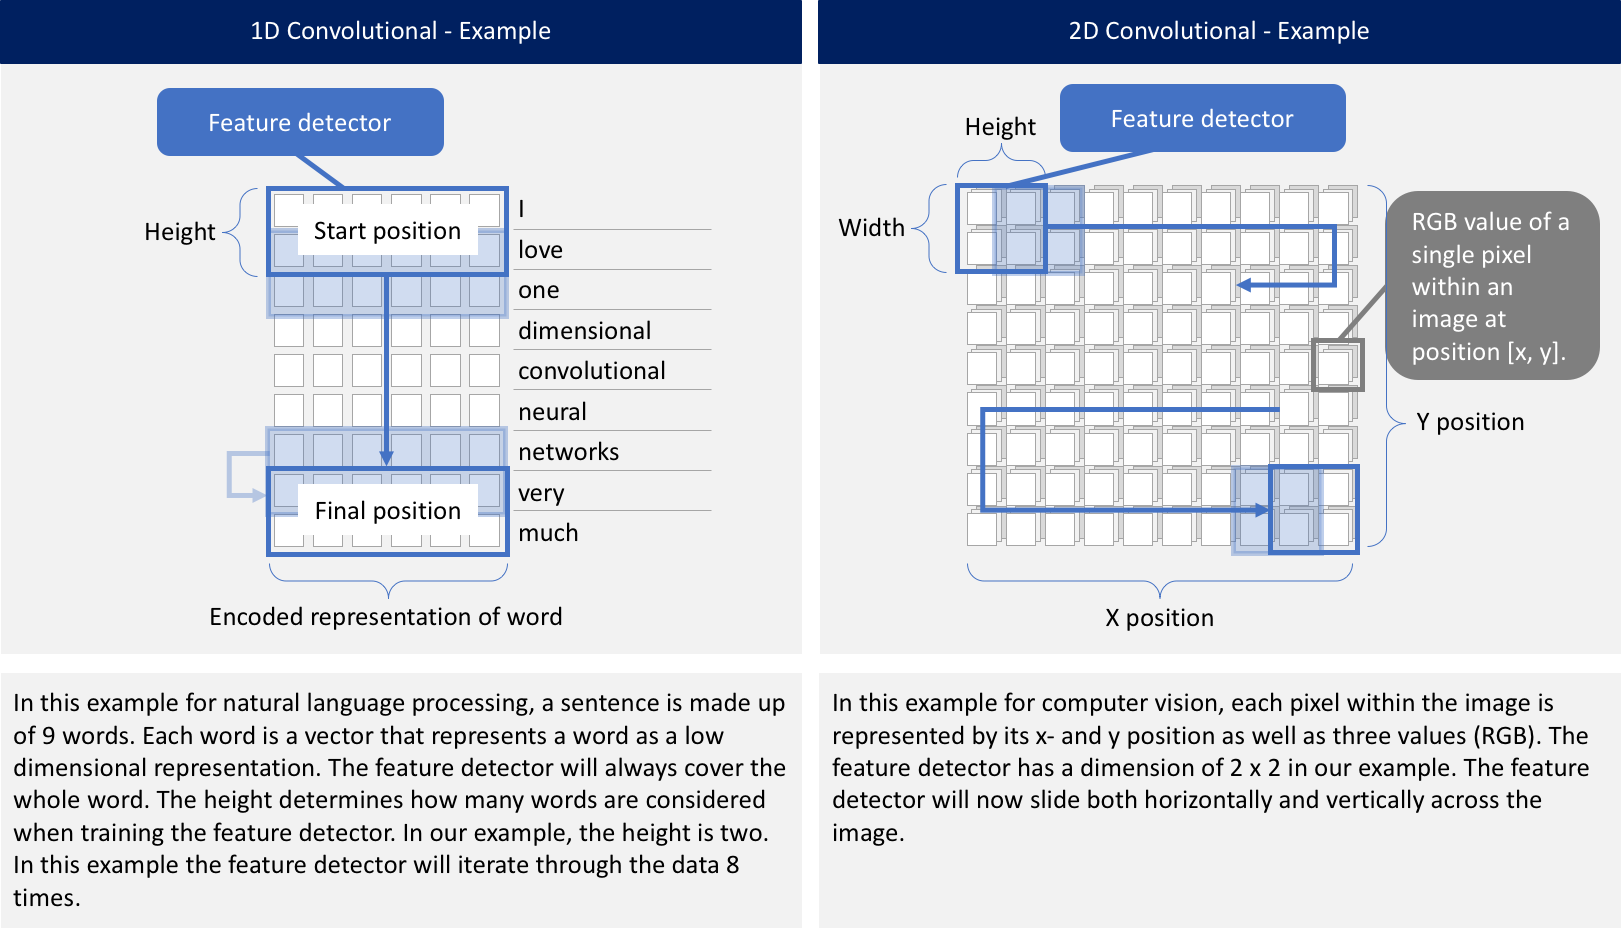
\includegraphics[scale=0.2]{conv1d}
\caption{Differenza convoluzione 1D e 2D}
\end{figure}

\subsection{Modello CNN proposto}
\todo{screen modello}

\subsection{CNN modulare}


\section{Dataset}
Come descritto nelle sezioni precedenti, l'allenamento delle reti neurali prevede l'utilizzo di un dataset. Si è scelto un allenamento di tipo supervisionato, pertanto il dataset necessita di valori di input e relativi output attesi, da confrontare con i risultati della rete. Il dataset utilizzato è quello del Children's Hospital Boston, che comprende EEG provenienti da 22 diversi pazienti pediatrici. Le misurazioni sono state effettuate con una frequenza di campionamento di 256 Hz e la maggior parte dei files contiene 23 canali. Per l'allenamento della rete è stata utilizzata solo una parte di questi files, in particolare sono stati selezionati files con almeno una crisi e con esattamente 23 segnali EEG provenienti dai pazienti 1 ,2, 3, 5, 7 e 8.

L'allenamento della rete è stato effettuato su finestre di 30 secondi di tempo. Per la creazione del dataset si sono seguiti i seguenti passi per ogni file:
\begin{itemize}
\item Isolamento segnali di crisi epilettica, in base ai secondi di inizio e fine crisi riportati nel file \textit{chbNN-summary.txt} di ogni paziente
\item Suddivisione dei segnali di crisi in finestre da 30 secondi, applicando uno stride di 1 secondo (overlapping 29 secondi tra una finestra e l'altra)
\item Eliminazione dei segnali pre e post ictali, scelti convenzionalmente 5 minuti prima e dopo la crisi. Questo per evitare di influenzare il dataset con segnali aventi parziali caratteristiche di crisi
\item Selezione di finestre non di crisi, in numero pari alle finestre di crisi calcolate in precedenza
\end{itemize}
\todo{Che altro aggiungere? }
\section{Structure Application}
L'applicazione creata è suddivisa in due grandi componenti, da una parte il backend che offre servizi e modella la struttura dei dati, dall'altra il frontend che richiede i servizi e ne implementa l'interfaccia grafica, in modo da garantire un'interazione user friendly con l'utente.
Questa garantisce anche una più facile manutenzione del codice, visto che ognuna delle due parti è divisa in diversi componenti.
L' aplicazione è una web app, essa infatti è capace di girare sia nell'ambito web che mobile grazie ai vari framework utilizzati.
Essa è una single page application, cioè un'applicazione web che è fruibile su una sola pagina web garantendo una fluidità maggiore nell'esperienza dell'utente.
\subsection{Funzionalità offerte}
\todo{anaisi, predizione, creazione rete allenamento...}
\section{Backend}
La parte di backend è utilizzabile indipendentemente dall'interfaccia fornita. Di seguito le librerie e i framework utilizzati e una descrizione delle API fornite. 
\subsection{Django Framework}
Django è un server-side web framework Python estremamente popolare. Un web framework è un insieme di componenti che rendono lo sviluppo di siti web più facile e veloce. 
Django aiuta a eliminare tutte quelle attività che vengono ripetute durante lo sviluppo dell'applicazione, rendendo il processo di sviluppo un'attività facile e rapida. 
Si tratta di un web framework di alto livello scritto in linguaggio Python, sviluppato dalla Django Software Foundation e distribuito open source. 
Essendo un framework di sviluppo web, quindi con un interfaccia web, si parla di un pattern alla base chiamato MVC, che corrisponde a tre componenti: Model, View e Controller.
Anche Django usa questo pattern, però nel suo caso il pattern è chiamato MVT, che corrispondono a tre componenti quali: Model, View, Template.
\begin{itemize}
\item Model: corrisponde a un insieme di classi python che descrivono il modello dei dati. Esse forniscono una rappresentazione delle tabelle del database, consentendo di sfruttare gli oggetti per effettuare operazioni CRUD sui dati. Le informazioni delle classi sono contenute nel file \textit{models.py}.


è la parte del programma che si occupa del database. Django fornisce una serie di comandi rapidi per la gestione delle operazioni più comuni.
\item Template: corrisponde nella vista dell'applicazione, consente di effettuare l'interazione con l'app web essa descrive tutti i componenti visuali facenti parte della GUI con cui l'utente poi andrà ad interagire.
Il Template consiste di file html che descrivono la presentazione dei dati implementando la \textit{View} del pattern. 

consiste in una serie di documenti per la generazione di codice HTML, combinando l'utilizzo di parti statiche e tag dinamici. In questo progetto non è stato tuttavia utilizzato alcun template, dato che la parte visuale è gestita esternamente dal framework Ionic. 
\item View: funzioni python che gestiscono il flusso di esecuzione dell'applicazione, implementando la parte del controller del pattern MVC. Garantisce la possibilità di creare delle pagine e di descriverne il comportamento che esse avranno in funzione dell'iterazione con l'utente.
La View descrive e modella il comportamento dell'intera applicazione, rispondendo a eventi scaturiti dall'interazione con l'utente e modellando i dati facente parti del modello


gestisce l'interazione tra utente, sistema e database. Si occupa di ricezione, elaborazione e risposta alle richieste dell'utente.
\end{itemize}
\begin{figure}[!h]
\centering
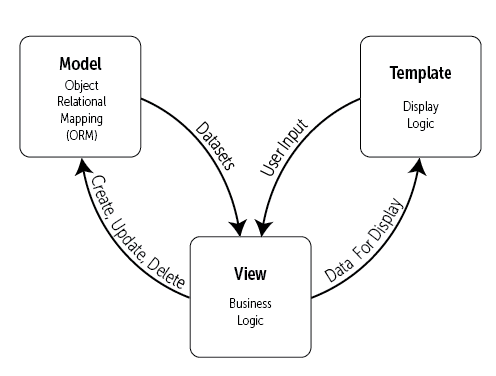
\includegraphics[scale=0.5]{mtv}
\caption{Relazioni modello MTV}
\end{figure}

\subsection{Python}
La sezione di backend del programma è stata scritta in Python, linguaggio di programmazione interpretato, di alto livello e generico.
Esso supporta diversi paradgmi di programmazione, come quella procedurale, orientata agli oggetti e funzionale. 
Di seguito verranno descritte le più importanti librerie utilizzate nel progetto.

\subsection{PyEDFlib}
Il funzionamento base del sistema prevede la lettura di tracciati EEG. Questi vengono comunemente distribuiti nel formato EDF (European Data Format), ideato per lo scambio di segnali multucanali fisici e biologici. La libreria che si occupa dell'interazione con tali file è PyEDFlib, basata a sua volta su edflib e Numpy. Essa mette a disposizione funzioni per la lettura dei segnali del file e dei suoi metadati, tra cui il numero di canali, la lunghezza e la frequenza del campionamento, l'inizio e la fine della rilevazione. 

\subsection{PyTorch}
La parte di neural network e deep learning è stata realizzata mediante l'utilizzo del framework PyTorch
PyTorch è una libreria del linguaggio Python basata sul framework torch.
Essa contiene diverse funzioni e metodi scientifici per le applicazioni dedicate al machine learning, al deep learning e al natural processing language.
PyTorch offre  due funzionalità di alto livello:
\begin{itemize}
\item Tensor Computing(come NumPy) con for vte accelerazione attraverso unità di elaborazione grafica(GPU)
\item Piattaforma di ricerca del deep learning che offre la massima flessibilità e  velocità \todo {da vedere}
\end{itemize}

\subsection{API}
L'utente ha la possibilità di interagire con il sistema attraverso richieste HTTP, ricevendo in risposta dei file in formato JSON. Di seguito sono descritte le principali Views messe a disposizione. Nelle successive sezioni verranno invece discusse le scelte riguardanti l'interfaccia grafica, che sfrutta queste views per fornire un'esperienza utente più facile e immediata anche per utenti poco esperti.
\paragraph{Single File analysis}
\begin{itemize}
\item \textit{/} [myfile]: upload del file mediante richiesta POST. Restituisce i parametri del file EDF caricato, come numero di canali, lunghezza, frequenza di campionamento. Solo dopo sver caricato il file è possibile fare richieste GET alle successive views.
\item \textit{/values} [channel, start, len]: ottiene i valori registrati in un determinato intervallo di tempo, provenienti da uno specifico canale. Restituisce la scala temporale in cui tali valori sono misurati. 
\item \textit{/complete}[start, len]: restituisce una finestra completa dell'EEG (quindi comprendente segnali di ogni canale) in uno specifico intervallo di tempo. 
\item \textit{/statistic}[channel]:relativamente ad uno specifico canale, calcola le statistiche dei segnali misurati, quali valore massimo e minimo, media, varianza e deviazione standard. 
\item \textit{/distribution}[channel]: relativamente ad uno specifico canale, restituisce due liste: una con intervalli di valori, e un'altra con il numero di segnali registrati in ogni intervallo. Con queste misure è possibile costruire un'istogramma che mostri la distribuzione dei valori. 
\item \textit{/predict}[model\textunderscore id]: effettua la predizione di crisi epilettiche sul file caricato. L'utente ha la possibilità di scegliere il modello da utilizzare, fornendone l'id. I segnali del file vengono suddivisi in finestre della dimensione accettata dal modello scelto. Per ogni finestra la rete restituirà la predizione sotto forma di 1 e 0 rispettivamente per segnale di crisi e non. Vengono inoltre restituiti il numero di finestre con crisi e il numero di finestre totali. 
\end{itemize}
\paragraph{Training}
\begin{itemize}
\item \textit{/uptraining} [myfile][seizureStart, seizureEnd]: caricamento dei files da utilizzare per l'allenamento della rete. Per ogni file l'utente deve specificare in quale intervallo di tempo si presenta la crisi. Vengono restituite le info sul file caricato e una lista di tutti i file finora caricati.
\item \textit{/cleanfiles}: cancella tutti i file di training finora caricati. 
\item \textit{/convert} [windowSize, stride]: converte tutti i file di training finora caricati in un dataset, con finestre della dimensione scelta. L'utente può inoltre scegliere un valore di stride da applicare alle finestre della crisi, in modo da ottenerne in numero maggiore. Questa view è necessaria prima di chiamare la view del training. La chiamata a questa view cancella tutti i files di training. \todo{come salvo i files}
\item \textit{/addconv}[output, kernel, stride, padding, pool\textunderscore kernel, pool\textunderscore stride]: permette l'aggiunta di un livello convoluzionale alla rete da creare. I parametri scelti dall'utente vengono salvati come record del database, dopo averne controllato la consistenza (evitare che l'output sia nullo, o che il kernel sia di dimensioni maggiori della finestra di segnali. Notare che insieme al layer convoluzionale l'utente specifica anche i parametri di un livello di MaxPool
\item \textit{/cleanlayers}: elimina tutti i livelli finora impostati.
\item \textit{initializenet}[linear]: crea un'istanza di rete pronta per essere allenata. I parametri venfono rirpesi dal database in ordine di inserimento. Viene automaticamente aggiunto un livello lineare finale che standardizzi l'output a due valori; l'utente ha inoltre la possibilità di aggiungere un ulteriore livello lineare impostando il parametro \textit{linear}.
\item \textit{/train} [epochs, train\textunderscore method]: crea una nuova rete e la allena sul dataset precendentemente creato. L'utente deve indicare il numero di epoche e quale metodo di validazione utilizzare. La validazione permette di prevenire l'overfitting dei dati, cioè che l'allenamento permetta alla rete di generalizzare il suo funzionamento. A tale scopo, vengono scelti dei dati da passare alla rete senza effettuare backpropagation. \'E possibile sccegliere il validation seti con diversi metodi. Ne sono stati implementati due:
\begin{itemize}
	\item k-fold training: all'interno di ogni epoca i segnali di un file vengono isolati, e passati alla rete dopo l'allenamento senza 	effettuare backpropagation. Nell'epoca successiva questi segnali faranno parte del dataset di allenamento, e verrà selezionato il file successivo per la validazione.
	\item k-window training: all'inizio di ogni epoca vengono selezionate randomicamente il 20\% delle finestre da utilizzare per la validazione.
\end{itemize}
Al termine dell'allenamento la rete viene salvata nel sistema, e sarà possibile utilizzarla per le predizioni. 
\item \textit{/usermodels]}: restituisce id e nome dei modelli creati attraverso il training. 
\item \textit{/cleanmodels}: elimina tutti i modelli in memoria. 
\end{itemize}


\section{Frontend}
La parte di frontend è stata implementata per garantire la gestione dell'interfaccia grafica che poi andrà ad interagire con l'utente, essa rappresenta il confine del sistema.

\subsection{Angular}
Angular è un framework javascript  per la scrittura di applicazioni web  client. Per raggiungere questo obiettivo, viene usato l'approccio dichiarativo dell'Html per quanto riguarda l'interfaccia grafica, e vengono forniti strumenti per costruire un'architettura modulare avente logica applicativa.
Un concetto fondamentale di angular sono i componenti, l'applicazione è formata da un insieme di componenti che interagiscono tra loro ed  hanno il controllo di una porzione dello schermo implementando una view.
il Framework supporta il pattern MVC.
il binding bidirezionale (two-way binding)
la dependency injection
il supporto al pattern MVC
il supporto ai moduli
la separazione delle competenze
la testabilità del codice
la riusabilità dei componenti
\subsection{Ionic}
Ionic framework è un toolkit  di interfaccia utente per la creazione di  applicazioni mobili e desktop performanti che utilizzano tecnologie web.
Ionic si concentra sull'esperienza utente di un'app (controlli, interazioni, gesti, animazioni). Esso si integra in modo facile a tecnologie come angular.
Il framework ionic consente di sviluppare app per tutte le piattaforme più comuni, come android, Ios e windows. Con Ionic risulta molto facile creare la parte di interfaccia grafica, che è molto vicina a quella nativa del dispositivo dove verrà eseguita l'app.
\subsection{HIghChart}
Highchart è una libreria grafica che permette di disegnare grafici a piacimento dello sviluppatore. e' capace di rappresentare grafici anche con grandi moli di dati.
\nocite{*}
\printbibliography[heading = bibintoc]
\end{document}